\section{Numerical simulations}\label{Section5}

En esta sección mostraremos algunos ejemplo resolviendo el problema de control óptimo mediante el método directo y la herramienta de optimización no lineal bajo constrain: CasADi \cite{Andersson2019}.
%
\subsection{Smooth approximation of piecewise linear penalization}

Con el fin de utilizar softwre de optimización para resolver el problema de control óptimo planteado aproximaremos penalización lineal a trozos mediante con ayuda de función escalón de Heaviside $h:\mathbb{R} \rightarrow \mathbb{R}$ y su aproximación suave $h^\eta:\mathbb{R} \rightarrow \mathbb{R}$ definida de la siguiente manera: 
\begin{gather}
    h(x) = \begin{cases}
        1 & \text{ if } x \geq 0 \\
        0 & \text{ if } x < 0
    \end{cases}    
    \hspace{2em} 
    \begin{cases}
        h^\eta(x) = (1 + \tanh(\eta x))/2   \\
        \eta \rightarrow \infty
    \end{cases}
\end{gather}
Con ayuda de la función $h$ definimos la función ventana suave $\Pi_{a,b}^\eta:\mathbb{R} \rightarrow \mathbb{R}$ como:
\begin{gather}
    \Pi_{[a,b]}^\eta(x) = - 1 + h^\eta(x-a) + h^\eta(-x+b) 
\end{gather}
De manera simplificada: 
\begin{gather}
    \Pi_{[a,b]}^\eta(x) = \frac{\tanh[\eta( x -a)] + \tanh[\eta (b-x)]}{2}
\end{gather}
De esta menera podemos escribir la versión  suave de (\ref{PLP}):
\begin{gather}
    \mathcal{L}^\eta(u) = \sum_{k = 1}^{N_u-1} \big[ (u_{k+1}+u_{k}) (u-u_k) + u_k^2 \big] \Pi^\eta_{[u_k,u_{k+1}]}(u)
\end{gather}
De manera que cuando $\eta \rightarrow \infty$ entonces $\mathcal{L}^\eta \rightarrow \mathcal{L}$

\subsection{Direct method  for  OCP-SHE}

To solve the optimal control problem (\ref{OCP2}), we use a direct method. 
%
If we consider a partition $\mathcal{P} = \{\tau_0,\tau_1,\dots,\tau_{T}\}$ of interval $[0,T]$ , we can represent a function $\{ u(\tau) \ | \ \tau \in [0,T]\}$ as a vector $\bm{u} \in \mathbb{R}^{T}$ where component $u_t = u(\tau_t)$. 
%
Then the optimal control problem (\ref{OCP1}) can be written as optimization problem with variable $\bm{u} \in \mathbb{R}^{T}$. This problem is a nonlinear programming, for this we use CasADi software to solve. 
%
Entonces, dado una partición del intervalo $[0,\pi)$ podemos reformular el problema (\ref{OCP1}) como el siguiente problema en tiempo discreto:
\newline
\begin{problem}[OCP numérico]
    Dados dos conjuntos de números impares $\mathcal{E}_a$ and $\mathcal{E}_b$ con cardinalidades $|\mathcal{E}_a| = N_a$ y  $|\mathcal{E}_b| = N_b$ respectivamente, dados los vectores objetivos $\bm{a}_T  \in \mathbb{R}^{N_a}$, de manera que $\bm{x}_0 = [\bm{a}_T,\bm{b}_T]^T$; y $\bm{b}_T  \in \mathbb{R}^{N_b}$ y una  partition $\mathcal{P}_\tau = \{\tau_0,\tau_1,\dots,\tau_{T}\}$ of interval $[0,\pi)$. We search a vector $\bm{u} \in \mathbb{R}^{T}$ that minimize the following function:
    \begin{gather}
        \min_{\bm{u} \in \mathbb{R}^{T} } 
        \Bigg[ 
        || \bm{x}^{T}||^2
        + \epsilon  \sum_{t=0}^{T-1} \mathcal{L}^\eta(u_{t}) \Delta\tau_t  \Bigg]  \\
        \notag \text{suject to: } \\
        \forall \tau \in \mathcal{P} \begin{cases}
            \bm{x}^{t+1} = \bm{x}^{t} - (2/\pi)\Delta \tau_t \bm{\mathcal{D}}(\tau_t)u_t \\
            \bm{x}^0 = \bm{x}_0
        \end{cases} 
    \end{gather}
\end{problem}



\subsection{Resultados}

Cabe mencionar que todas las simulaciones se han realizado con un ordenador de mesa con $8Gb$ de ram, y el tiempo de ejecución para la búsqueda de soluciones dado un vector objetivo es del orden del segundo. A continuación listaremos cada uno de los resultados numéricos obtenidos:
\begin{enumerate}    


    \item \textbf{OCP con simetría de cuarto de onda}: Consideraremos el problema  con un conjunto de números impares $\mathcal{E}_b = \{1,5\}$ con una discretización del intervalo $[0,\pi/2]$ de $T = 200$. Mostramos las soluciones para los vectores objetivo $b_T^1 = \{(-0.4,-0.3,\dots,0.3,0.4)\}$ manteniendo $b_T^5=0$ para todos los casos. Mostramos las trayectorias óptimas obtenidas en la figura (\ref{ex01}), donde se puede ver una continuidad en las soluciones con respecto a vector objetivo.

    % \begin{figure}
    %     \centering
    %     \begin{subfigure}[b]{\textwidth}
    %         \centering
    %         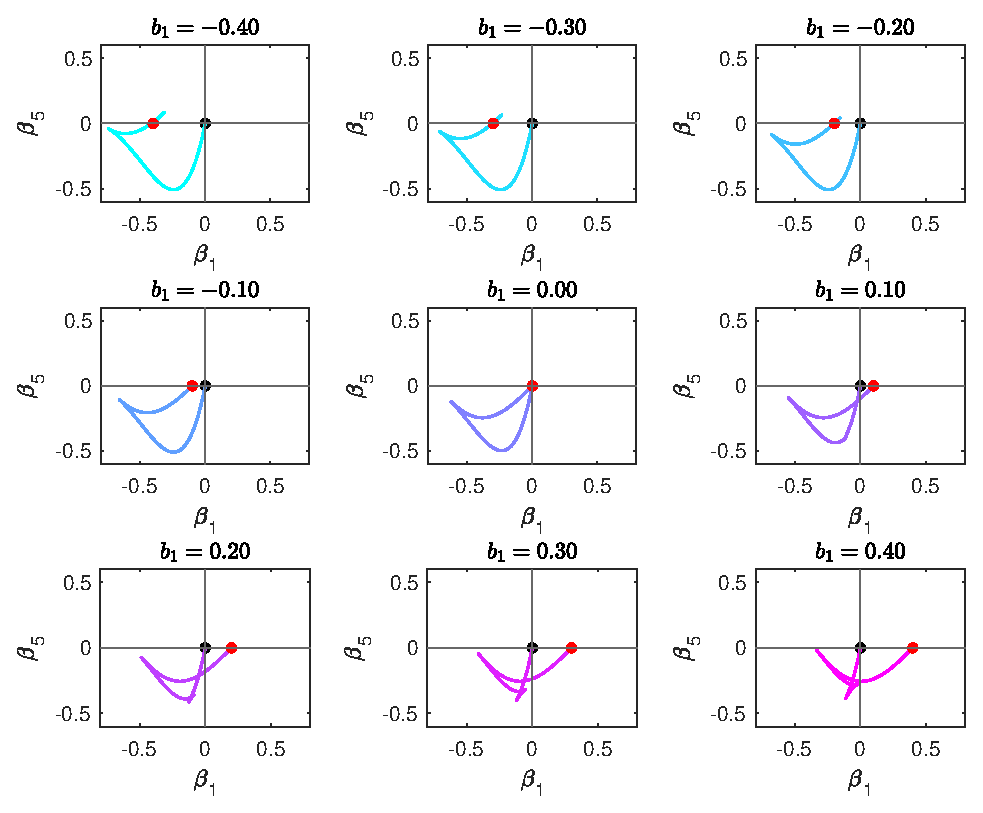
\includegraphics[width=0.6\textwidth]{img/ex01-con.eps}
    %         \caption{Dynamical System: el punto rojo hace referencia al punto final mientras que el punto negro hace referencia al punto inicial.}
    %     \end{subfigure} 
    %     \hfill \\
    %     \begin{subfigure}[b]{\textwidth}
    %         \centering
    %         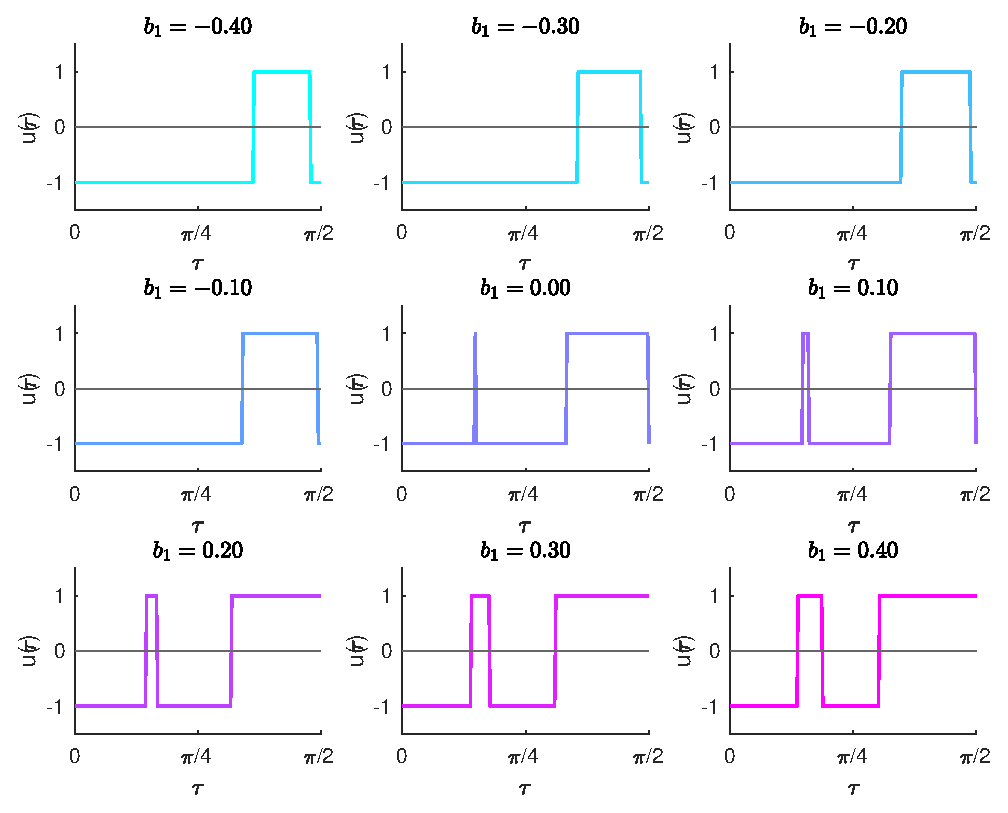
\includegraphics[width=0.6\textwidth]{img/ex01-dyn.eps} 
    %         \caption{Control}
    %     \end{subfigure}
    %     \caption{Mostramos las trayectorias óptimas y controles óptimos para distintos vectores objetivo.}
    %     \label{ex01}
    % \end{figure}


    \item \textbf{OCP con simetría de cuarto onda para un intervalo del $b_1$}: Para este ejemplo consideramos el siguiente conjunto de números impares: $\mathcal{E}_b = \{1,5,7,11,13\}$. 
    %
    Ademas consideramos el vector objetivo $\bm{b}_T = [m_a,0,0,0,0]$, donde  $m_a \in [-1,1]$ es un parámetro. with three penalization terms: $\mathcal{L}(u) = -f$, $\mathcal{L}(u) = +f$ and $\mathcal{L}(u) = -f^2$ obtained by direct method with uniform partition of interval $[0,\pi/2]$ with $T=400$ and penalization parameter $\epsilon = 10^{-5}$. 
    %
    Para cada uno de los términos de penalización utilizados la distancia entre los coeficientes de Fourier se encuentra en el orden de $10^{-4}$. 
    %
    Sin embargo, cuando el término de penalización es $\mathcal{L}(u)= -f^2$ la solución no presenta continudad con respecto al vector objetivo. 
    %
    Por otra parte, es importante mencionar que las soluciones para los términos de penalización $\mathcal{L}(u) = -f$ y $\mathcal{L}(u) = f$ cumplen una simetría por lo que invirtiendo las soluciones con respecto al origen y invirtiendo el signo de las soluciones se puede ver que ambas soluciones son la misma.


     
    \item \textbf{SHE para tres niveles}: Podemos ver que en el caso en el que el control $u(\tau)$ solo pueda tomar valores entre $[0,1]$ obtenemos señales que pueden tomar tres niveles en el intervalo $[0,2\pi]$ gracias a la simetría de cuarto de onda. Si resolvemos el problema de control óptimo pero esta vez cambiando las restricciones $|u(\tau)|<1$ por $\{0<u(\tau)<1\}$. Se ha realizado el mismo procedimiento que en el caso anterior, obteniendo soluciones para los mismo términos de penalización obteniendo la figura (\ref{ex3LVL}). Allí se muestra la continudad de las soluciones y que estas se encuentran en el orden de $10^{-4}$.
    



    
      


    \item \textbf{Cambio en el número de conmunationes}: Gracias a la formulación de control óptimo para el problema SHE podemos variar el número de ángulos de conmuntación. 
    %
    Este es el cado del siguientes ejemplo, donde hemos tomado como conjunto de números pares $\mathcal{E}_b = \{1,3,9,13,17\}$,   además consideramos el vector objetivo $\bm{b}_T = [m_a,0,0,0,0]$, donde  $m_a \in [0,1]$ es un parámetro. 
    %
    En este problema hemos utilizado una penalización tipo $\mathcal{L} = f$ con un parémetro de penalización $\epsilon=10^{-4}$.
    %
    Podemos ver en la figura (\ref{disco}) como el problema de control óptimo es versátil y es capaz de mover entre varios conjuntos de soluciones.




    
    \item \textbf{OCP para SHE con simetría de media onda}: Se ha relizado el caso de control óptimo de media onda con con $\mathcal{E}_a = \{1,3,5\}$ y  $\mathcal{E}_b = \{1,3,5,9\}$, donde $\bm{a}_T = [m_a,0,0]$, $\bm{b}_T = [m_a,m_a,0,0]$ y  $m_a \in [-0.6,0.6]$. Se ha elegido la penalización $L(u) = +f$



\end{enumerate}






